\documentclass[border=6pt]{standalone}
\usepackage{tikz}
\usetikzlibrary{arrows.meta,positioning,calc,shapes.geometric,fit,backgrounds,patterns,matrix,decorations.pathreplacing}
\begin{document}
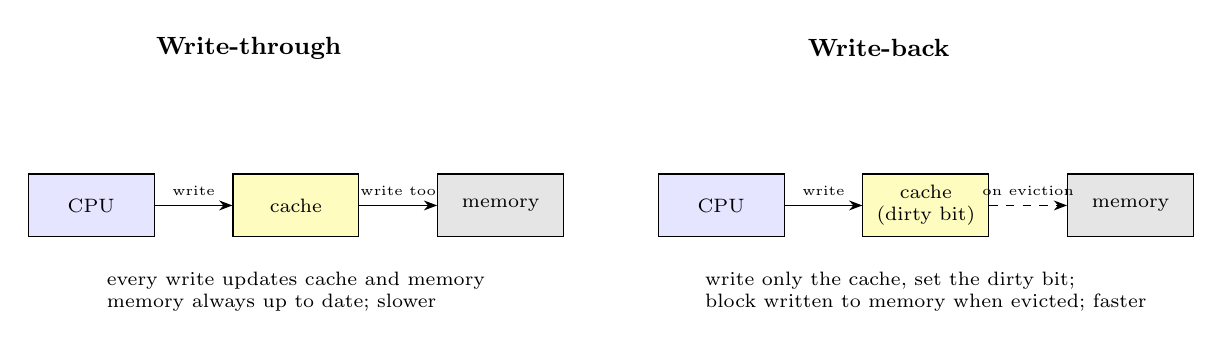
\begin{tikzpicture}[>=Stealth,font=\small]
\tikzstyle{b}=[draw,minimum height=0.8cm,minimum width=1.6cm,align=center,font=\scriptsize]
\node[font=\small\bfseries] at (2,2) {Write-through};
\node[b,fill=blue!10] (c1) at (0,0) {CPU}; \node[b,fill=yellow!25] (k1) at (2.6,0) {cache}; \node[b,fill=gray!20] (m1) at (5.2,0) {memory};
\draw[->] (c1) -- node[above,font=\tiny]{write} (k1); \draw[->] (k1) -- node[above,font=\tiny]{write too} (m1);
\node[font=\scriptsize,align=left] at (2.6,-1.1) {every write updates cache and memory\\ memory always up to date; slower};
\node[font=\small\bfseries] at (10,2) {Write-back};
\node[b,fill=blue!10] (c2) at (8,0) {CPU}; \node[b,fill=yellow!25] (k2) at (10.6,0) {cache\\ (dirty bit)}; \node[b,fill=gray!20] (m2) at (13.2,0) {memory};
\draw[->] (c2) -- node[above,font=\tiny]{write} (k2); \draw[->,dashed] (k2) -- node[above,font=\tiny]{on eviction} (m2);
\node[font=\scriptsize,align=left] at (10.6,-1.1) {write only the cache, set the dirty bit;\\ block written to memory when evicted; faster};
\end{tikzpicture}
\end{document}
